\documentclass{beamer}
\usepackage[size=custom, width=21, height=28, scale=1.0, orientation=portrait]{beamerposter}
\setbeamertemplate{navigation symbols}{}
\setbeamersize{text margin left=0em,text margin right=0em}

\usepackage{tikz}
\usetikzlibrary{positioning}
\usetikzlibrary{calc}
\usetikzlibrary{arrows,positioning, decorations, decorations.text}

% use Helvetica font
\usepackage{fontspec}
\usefonttheme{serif}
\usepackage{helvet}

\usepackage{graphicx}
\graphicspath{{../}}

%----------------------------------------------------------------------------------------
\begin{document}

% Needed to set equation counter, following inclusion of figure 1
\setcounter{equation}{2}

\begin{tikzpicture}[remember picture, overlay]

\newcommand{\rowspace}{3}
\newcommand{\colspace}{3.5}

\newcommand{\plot}[2]{
  \node[anchor=center, rectangle]
    at (#1) {\includegraphics[height=1.85cm]{#2}};
}

\newcommand{\ylabel}[2]{
  \node at (#1)[anchor=west, text width=2cm, minimum height=1cm] {
  {\footnotesize #2}};
}

\newcommand{\textbox}[2]{
  \node at (#1)[anchor=center] {
  {\footnotesize #2}};
}

\newcommand{\defineRow}[2]{
  \node at ($(top) + (-9.5cm, -#1*\rowspace cm)$) (#2){};
}

\newcommand{\defineCol}[3]{
  \node at ($(#1) + (#2*\colspace cm, 0cm)$) (#3){};
}


\newcommand{\rowtitle}[1]{
  \node at ($(thisrow) + (0.25cm, 1.5cm)$) [anchor=west, text width=12cm, text height=0.5cm]{
  {\bf \footnotesize #1}};
}

\newcommand{\rowlabel}[1]{
  \node at ($(thisrow) + (-0.75cm, -0.3cm)$)[anchor=west, text width=2cm] {
 {\color{black!30}\begin{equation}\label{#1}\end{equation}}};
}

\newcommand{\firstcol}[4]{
  \defineCol{thisrow}{#1}{thiscol}
  \ylabel{$(thiscol) + (-2.1cm,  0cm)$}{#2}
  \plot{  $(thiscol)$                 }{#3}
  \ylabel{$(thiscol) + (0.7cm,   0cm)$}{=}
  \ylabel{$(thiscol) + (1.1cm,   0cm)$}{#4}
}

\newcommand{\othercol}[4]{
  \defineCol{thisrow}{#1}{thiscol}
  \ylabel{$(thiscol) + (-2.1cm,   0cm)$}{#2}
  \plot{  $(thiscol)$                  }{#3}
  \ylabel{$(thiscol) + (0.85cm,   0cm)$}{#4}
}

\node at ($(current page.north)+ (0cm, -7.5cm)$) (top){};

\node[rectangle, anchor = center] at ($(top)+ (0cm, 4cm)$){
  \includegraphics[width=18cm]{output/main/mass_fraction.pdf}};

\node at ($(top) + (-9.25cm, 6.75cm)$) [anchor=west, text width=12cm, text height=0.5cm]{
  {\bf \footnotesize Standing mass}};

\node at ($(top) + (-10.5cm, 6.75cm)$) [anchor=west, text width=12cm, text height=0.5cm]{
  {\bf \footnotesize a)}};

\node at ($(top) + (-10.5cm, 1.5cm)$) [anchor=west, text width=12cm, text height=0.5cm]{
  {\bf \footnotesize b)}};

% \node[rectangle, anchor =center] at ($(top)+ (6cm, 4cm)$){
%   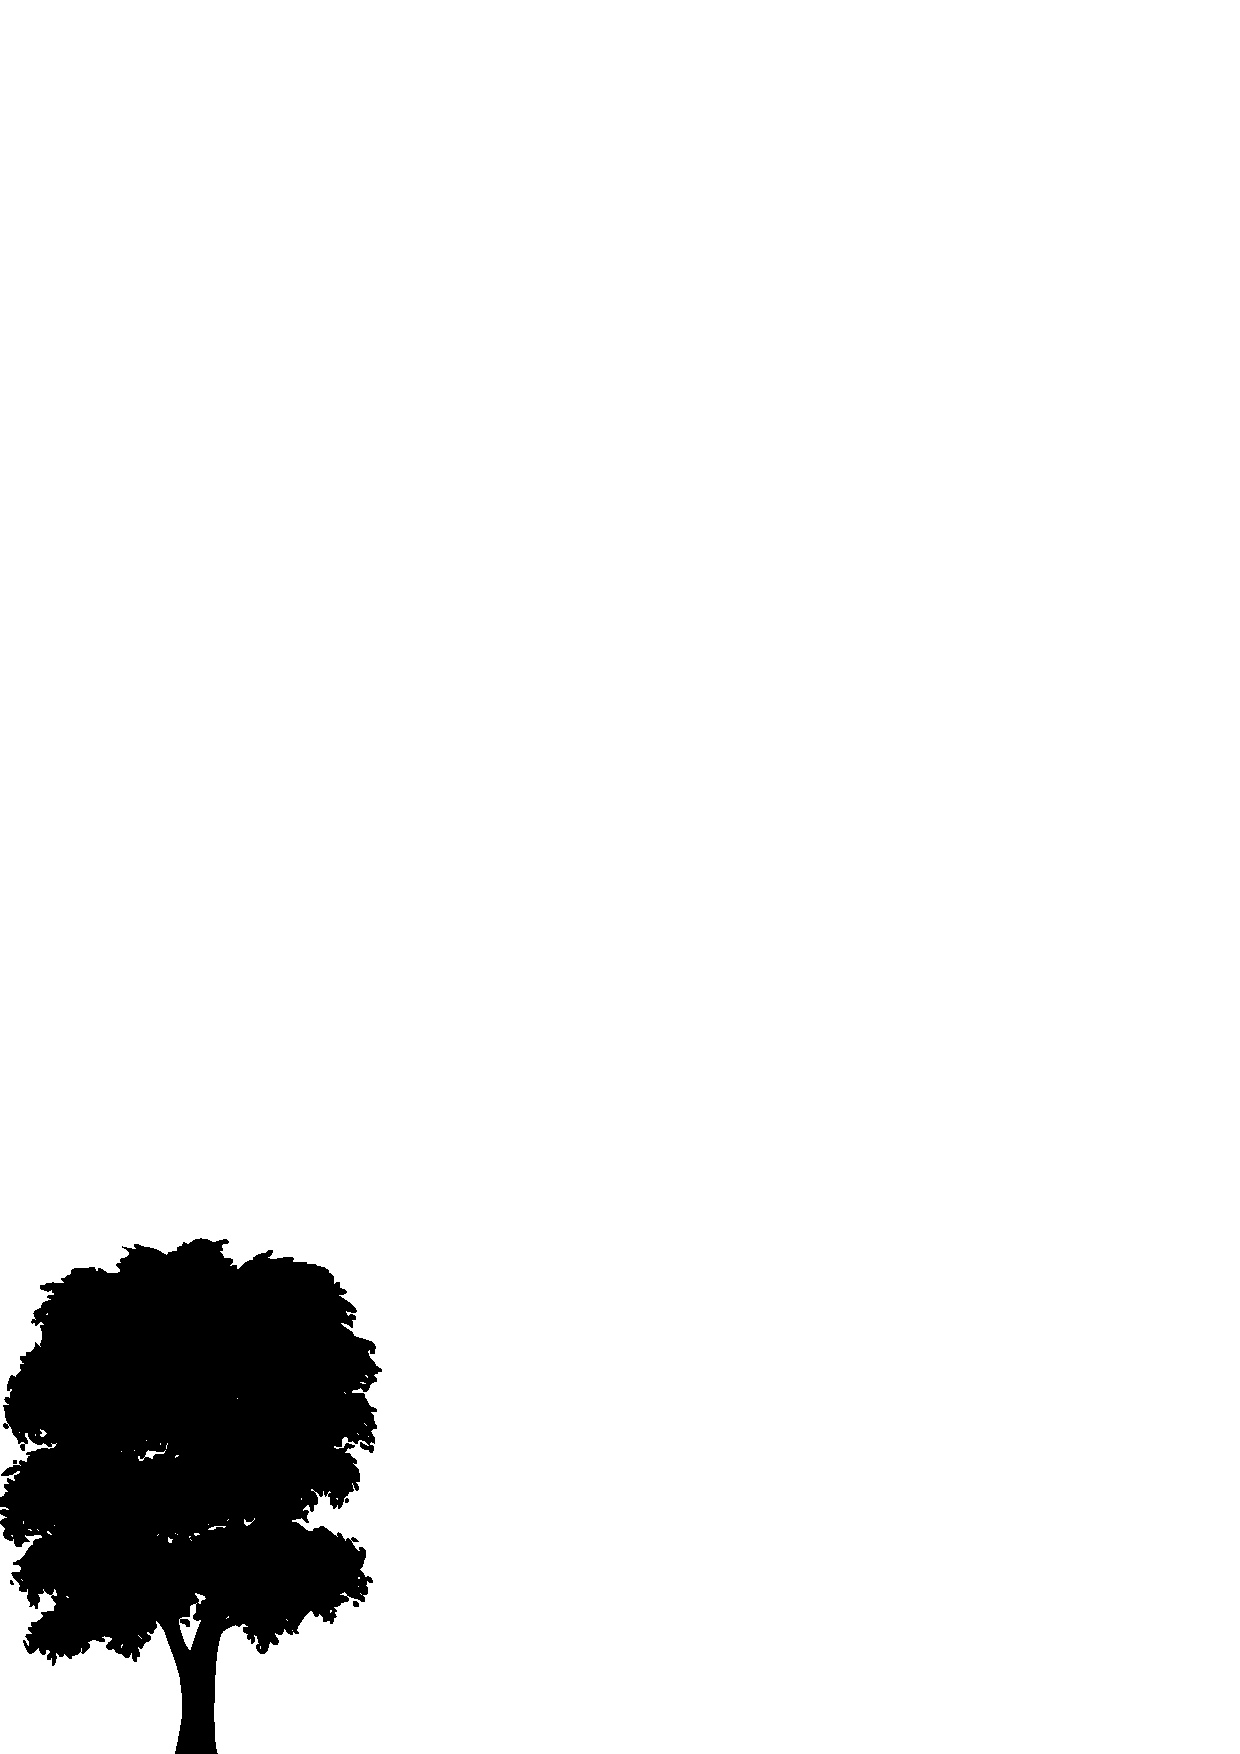
\includegraphics[height= 3cm]{downloads/tree.png}};
%   \textbox{$(top)+ (8.5cm, 4cm)$}{Adult}
% \node[rectangle, anchor =center] at ($(top)+ (-6cm, 4cm)$){
%   \includegraphics[height= 1cm]{downloads/seedling.png}};
%   \textbox{$(top)+ (-8cm, 4cm)$}{Seedling}

\defineRow{0}{thisrow}
\rowtitle{Biomass production}
\firstcol{1}{$\frac{{\rm d}B}{{\rm d}t}$}{output/con/net_mass_production_dt_net_mass_production_dt}{}
\othercol{2}{\hspace{-1em} \scriptsize $\alpha_{\rm \tiny bio} \alpha_{\rm \tiny y}$}{output/con/net_mass_production_dt_yield}{}
\othercol{3}{\hspace{-1em}$\times\Bigg($\hspace{-0.3em}\scriptsize$A_{\rm l} \bar{p}$}{output/con/net_mass_production_dt_assimilation}{}
\othercol{4}{\hspace{-1em}-$\Sigma$\scriptsize $M_{\rm i} r_{\rm i}$}{output/con/net_mass_production_dt_respiration}{\hspace{-0.5em}$\Bigg)$}
\othercol{5}{\hspace{-0.75em}-$\Sigma$\scriptsize $M_{\rm i} k_{\rm i}$}{output/con/net_mass_production_dt_turnover}{}
\rowlabel{eq:dbdt_2}

\defineRow{1}{thisrow}
\rowtitle{Mass growth}
\firstcol{1}{$\frac{{\rm d}M_{{\rm t}}}{{\rm d}t}$}{output/con/mass_total_dt_mass_total_dt}{}
\othercol{2}{$\frac{{\rm d}M_{{\rm a}}}{{\rm d}B}$}{output/con/mass_total_dt_fraction_allocation_growth}{$\times$}
\othercol{3}{$\frac{{\rm d}B}{{\rm d}t}$}{output/con/mass_total_dt_net_mass_production_dt}{$+$}
\othercol{4}{$\frac{{\rm d}M_{{\rm h}}}{{\rm d}t}$}{output/con/mass_total_dt_mass_heartwood_dt}{}
\rowlabel{eq:dMtdt}

\defineRow{2}{thisrow}
\rowtitle{Leaf deployment per mass invested}
\firstcol{1}{$\frac{{\rm d}A_{{\rm l}}}{{\rm d}M_{{\rm a}}}$}{output/con/darea_leaf_dmass_live_darea_leaf_dmass_live}{$\Bigg($}
\othercol{2}{$\frac{{\rm d}M_{{\rm l}}}{{\rm d}A_{{\rm l}}}$}{output/con/darea_leaf_dmass_live_dmass_leaf_darea_leaf}{+}
\othercol{3}{$\frac{{\rm d}M_{{\rm r}}}{{\rm d}A_{{\rm l}}}$}{output/con/darea_leaf_dmass_live_dmass_root_darea_leaf}{+}
\othercol{4}{$\frac{{\rm d}M_{{\rm b}}}{{\rm d}A_{{\rm l}}}$}{output/con/darea_leaf_dmass_live_dmass_bark_darea_leaf}{+}
\othercol{5}{$\frac{{\rm d}M_{{\rm s}}}{{\rm d}A_{{\rm l}}}$}{output/con/darea_leaf_dmass_live_dmass_sapwood_darea_leaf}{$\Bigg)^{-1}$}
 \rowlabel{eq:daldmt}

\defineRow{3}{thisrow}
\rowtitle{Leaf-area growth}
\firstcol{1}{$\frac{{\rm d}A_{{\rm l}}}{{\rm d}t}$}{output/con/area_leaf_dt_area_leaf_dt}{}
\othercol{2}{$\frac{{\rm d}A_{{\rm l}}}{{\rm d}M_{{\rm a}}}$}{output/con/area_leaf_dt_darea_leaf_dmass_live}{$\times$}
\othercol{3}{$\frac{{\rm d}M_{{\rm a}}}{{\rm d}B}$}{output/con/area_leaf_dt_fraction_allocation_growth}{$\times$}
\othercol{4}{$\frac{{\rm d}B}{{\rm d}t}$}{output/con/area_leaf_dt_net_mass_production_dt}{}
\rowlabel{eq:daldt}

\defineRow{4}{thisrow}
\rowtitle{Height growth}
\firstcol{1}{$\frac{{\rm d}H}{{\rm d}t}$}{output/con/height_dt_height_dt}{}
\othercol{2}{$\frac{{\rm d}H}{{\rm d}A_{{\rm l}}}$}{output/con/height_dt_dheight_darea_leaf}{$\times$}
\othercol{3}{$\frac{{\rm d}A_{{\rm l}}}{{\rm d}t}$}{output/con/area_leaf_dt_area_leaf_dt}{}
\rowlabel{eq:dhdt}

\defineRow{5}{thisrow}
\rowtitle{Stem-area growth}
\firstcol{1}{$\frac{{\rm d}A_{{\rm st}}}{{\rm d}t}$}{output/con/area_stem_dt_area_stem_dt}{$\Bigg($}
\othercol{2}{$\frac{{\rm d}A_{{\rm b}}}{{\rm d}A_{{\rm l}}}$}{output/con/area_stem_dt_darea_bark_darea_leaf}{$+$}
\othercol{3}{$\frac{{\rm d}A_{{\rm s}}}{{\rm d}A_{{\rm l}}}$}{output/con/area_stem_dt_darea_sapwood_darea_leaf}{\hspace{-0.3em}$\Bigg)$}
\othercol{4}{\hspace{-0.4em}$\times\frac{{\rm d}A_{{\rm l}}}{{\rm d}t}$}{output/con/area_stem_dt_area_leaf_dt}{$+$}
\othercol{5}{$\frac{{\rm d}A_{{\rm h}}}{{\rm d}t}$}{output/con/area_stem_dt_area_heartwood_dt}{}
\rowlabel{eq:dast}

\defineRow{6}{thisrow}
\rowtitle{Stem-diameter growth}
\firstcol{1}{$\frac{{\rm d}D}{{\rm d}t}$}{output/con/diameter_stem_dt_diameter_stem_dt}{}
\othercol{2}{$\frac{{\rm d}D}{{\rm d}A_{{\rm st}}}$}{output/con/diameter_stem_dt_ddiameter_stem_darea_stem}{$\times$}
\othercol{3}{$\frac{{\rm d}A_{{\rm st}}}{{\rm d}t}$}{output/con/diameter_stem_dt_area_stem_dt}{}
\rowlabel{eq:dDdt}

\textbox{$(top)+ (0cm, -20cm)$}{{\bf Plant height (m)}}

\newcommand{\colNum}{0.1}

\defineRow{0}{rowZero}
\defineCol{rowZero}{\colNum}{A}

\defineRow{1}{rowOne}
\defineCol{rowOne}{\colNum}{B1}

\defineRow{2}{rowTwo}
\defineCol{rowTwo}{\colNum}{B}

\defineRow{3}{rowThree}
\defineCol{rowThree}{\colNum}{C}

\defineRow{4}{rowFour}
\defineCol{rowFour}{\colNum}{D}

\defineRow{5}{rowFive}
\defineCol{rowFive}{\colNum}{E}

\defineRow{6}{rowSix}
\defineCol{rowSix}{\colNum}{F}

\tikzstyle{s1}=[->,line width=2pt, draw=black!20]

\draw [s1] (A) to [bend right, looseness=0.75] (C);
\draw [s1] (A) to [bend right] (B1);
\draw [s1] (B) to [bend right] (C);
\draw [s1] (C) to [bend right, looseness=0.75] (D);
\draw [s1] (C) to [bend right, looseness=1] (E);
\draw [s1] (E) to [bend right, looseness=1] (F);

\end{tikzpicture}
\end{document}